\documentclass[11pt,a4paper]{article}

\usepackage[margin=1in, paperwidth=8.3in, paperheight=11.7in]{geometry}
\usepackage{amsmath,amsfonts,fancyhdr,bbm,tikz}
\usetikzlibrary{trees}
\usepackage[section,nohyphen]{DomH}
\headertitle{Finance Mathematics - Problem Sheet 7}

\begin{document}

\questionsfalse
% \answersfalse

\title{Finance Mathematics - Problem Sheet 7}
\author{Dom Hutchinson}
\date{\today}
\maketitle

\begin{question}{1.}
  Consider a European call option with exercise price $e=1,000$ under the Cox-Ross-Rubinstein model with $T=2$ periods, $u=1.1$, $d=0.9$ and interest rate $r=0.01$. Show that the time $t=0$ option price is a piecewise linear function of the initial stock price $S_0$ and sketch a graph of the function.
\end{question}

\begin{answer}{1.}
  \everymath={\displaystyle}
  Define the probability $q$ st
  \[ q=\frac{1+r-d}{u-d}={1+0.01-0.9}{1.1-0.9}=\frac{11}{20} \]
  For this European call option, we have that the payoff function is
  \[ g(x)=\{x-e\}_+=\{x-1000\}_+ \]
  Under the Cox-Ross-Rubinstein model we have the time $t=0$ price of this option is
  \[\begin{array}{rrl}
    \Pi_e(0)&:=&\frac{1}{(1+r)^2}\left\{\sum_{n=0}^T{T\choose n}q^n(1-q)^{T-n}g(S_0u^nd^{T-n})\right\}\\
    &=&\frac1{1.01^2}\left\{\sum_{n=0}^2{2\choose n}\left(\frac{11}{20}\right)^n\left(\frac{8}{20}\right)^{T-n}\left(S_0\left(\frac{11}{10}\right)^n\left(\frac{9}{20}\right)^{T-n}-1000\right)\right\}\\
    &=&\frac1{1.01^2}\Bigg\{{2\choose2}\left(\frac{11}{20}\right)^2\left(S_0\left(\frac{11}{10}\right)^2-1000\right)+{2\choose1}\frac{11}{20}\cdot\frac{9}{20}\left(S_0\frac{11}{10}\cdot\frac9{10}-1000\right)\\
    &+&{2\choose0}\left(\frac{9}{20}\right)^2\left(S_0\left(\frac{9}{20}\right)^2-1000\right)\Bigg\}\\
    &=&\left(\frac{1}{1.01^2}\right)\left(\frac1{400}\right)\cdot\left\{121\left(S_0\frac{121}{100}-1000\right)+198\left(S_0\frac{99}{100}-1000\right)+81\left(S_0\frac{81}{100}-1000\right)\right\}
  \end{array}\]
  By inspection, each term of this function is clearly piecewise-linear wrt the initial price $S_0$.
  % TODO - graph
\end{answer}

\begin{question}{2.}
  Consider a Cox-Ross-Rubinstein model with $T=3$ periods, $S_0=100$, $u=1.6$ and $d=0.6$. The interest rate is $r=0.1$. What is the time $t=0$ price of an American put option with exercise price $e=90$?
  \par Show that it is only optimal to exercise early in the case that the stock falls twice in the first two moves.
\end{question}

\begin{answer}{2.}
  Consider the tree below which shows the possible evolutions of the price process $S_t$ for each time-point and event.
  \begin{center}
    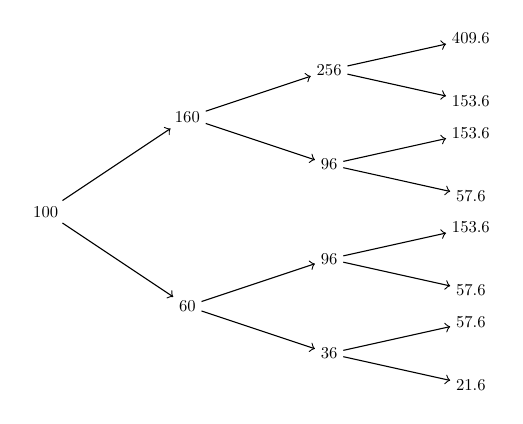
\begin{tikzpicture}[->, level/.style={sibling distance = 4cm/(#1), level distance = 3cm}, scale=0.6,transform shape,grow=right]
      \node {100}
        child {node {60}
          child {
            node {36}
            child {node {21.6}}
            child {node {57.6}}
          }
          child {
            node {96}
            child {node {57.6}}
            child {node {153.6}}
          }
        }
        child {node {160}
          child {
            node {96}
            child {node {57.6}}
            child {node {153.6}}
          }
          child {
            node {256}
            child {node {153.6}}
            child {node {409.6}}
          }
        };
    \end{tikzpicture}
  \end{center}
  For this American put option we have that the pay-out is $Y_t(\omega)=\{90-S_t(\omega)\}_+$ for each $t=0,1,2,3$ and $\omega\in\Omega$. I summarise the pay-outs in the tree below
  \begin{center}
    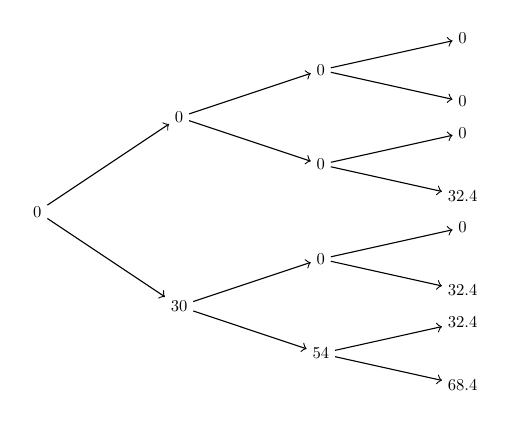
\begin{tikzpicture}[->, level/.style={sibling distance = 4cm/(#1), level distance = 3cm}, scale=0.6,transform shape,grow=right]
      \node {0}
        child {node {30}
          child {
            node {54}
            child {node {68.4}}
            child {node {32.4}}
          }
          child {
          node {0}
          child {node {32.4}}
          child {node {0}}
          }
        }
        child {node {0}
          child {
            node {0}
            child {node {32.4}}
            child {node {0}}
          }
          child {
            node {0}
            child {node {0}}
            child {node {0}}
          }
        };
    \end{tikzpicture}
  \end{center}
  We can calculate the probability value $q$ where
  \[ q:=\frac{1+r-d}{u-d}=\frac{1+0.1-0.6}{1.6-0.6}=\frac12 \]
  This means the probability of the price increasing and the probability price decreasing during each time period are both 1/2.
  \par I will now construct a Snell Envelope $\{Z_t\}$ for $\{Y_t\}$.
  \par By defintiion $Z_3(\omega)=Y_3(\omega)\ \forall\ \omega\in\Omega$.
  \par Let $\omega_{ud}$ denote the events where the price increased once and decreased once (in some order) during the first two time-steps and $\omega_{dd}$ denote the events where the price decreased twice during the first two time-steps. Note these are disjoint and that no other events can lead to a profitable payout.
  \par Suppose $t=2$ and $\omega_{ud}$ occurred. Then
  \[\begin{array}{rrcl}
    &\expect[Z_3|\mathcal{F}_2]&=&q\cdot0+(1-q)\cdot32.4\\
    &&=&\frac12(0+32.4)\\
    &&=&16.2\\
    \implies&Z_2(\omega_{ud})&=&\max\{Y_2(\omega_{ud}),\expect[Z_3,\mathcal{F}_2]\}\\
    &&=&\max\{0,16.2\}\\
    &&=&16.2
  \end{array}\]
  \par Suppose $t=2$ and $\omega_{dd}$ occurred. Then
  \[\begin{array}{rrcl}
    &\expect[Z_3|\mathcal{F}_2]&=&\frac12(32.4+68.4)=50.4\\
    \implies&Z_2(\omega_{dd})&=&\max\{Y_2(\omega_{dd}),\expect[Z_3,\mathcal{F}_2]\}\\
    &&=&\max\{54,50.4\}\\
    &&=&54
  \end{array}\]
  Let $\omega_u$ denote the events where the price increased during the first time-step and $\omega_d$ denote the events where the price decreases during the first time-step.
  \par Suppose $t=1$ and $\omega_{u}$ occurred. Then
  \[\begin{array}{rrcl}
    &\expect[Z_2|\mathcal{F}_1]&=&\frac12(0+16.2)=8.1\\
    \implies&Z_1(\omega_{u})&=&\max\{Y_1(\omega_{u}),\expect[Z_2,\mathcal{F}_1]\}\\
    &&=&\max\{0,8.1\}\\
    &&=&8.1
  \end{array}\]
  \par Suppose $t=1$ and $\omega_{d}$ occurred. Then
  \[\begin{array}{rrcl}
    &\expect[Z_2|\mathcal{F}_1]&=&\frac12(16.2+54)=35.1\\
    \implies&Z_1(\omega_{d})&=&\max\{Y_1(\omega_{d}),\expect[Z_2,\mathcal{F}_1]\}\\
    &&=&\max\{30,35.1\}\\
    &&=&35.1
  \end{array}\]
  \par Suppose $t=0$. Then
  \[\begin{array}{rrcl}
    &\expect[Z_1|\mathcal{F}_0]&=&\expect[Z_1]\\
    &&=&\frac12(8.1+35.1)\\
    &&=&21.6\\
    \implies&Z_0&=&\max\{Y_0,\expect[Z_1,\mathcal{F}_0]\}\\
    &&=&\max\{0,21.6\}\\
    &&=&21.6
  \end{array}\]
  The time $t=0$ fair-price of this American put is 21.6.
  \par By inspecting the calculations of each $Z_t$ above, the only time-point $t<3$ where $Z_t(\omega)=Y_t(\omega)$ is when $t=2$ and $\omega=\omega_{dd}$.
  \par Thus, the only scenario where exercising early is optimal is when the price falls twice in the first two time-periods.
\end{answer}

\begin{question}{3.}
  A stock price is currently £40. Over each of the next two three-month periods it will go up by 10\% or down by 8\%. The risk-free interest rate is 12\% per annum with continuous compounding. What is the value pf
\end{question}

\begin{question}{3. a)}
  A six-month European put option with strike price of £42?
\end{question}

\begin{answer}{3. a)}
  Note that the interest rate for a three month period is $r=0.03$.
  Consider the tree below which shows the possible evolutions of the price process $S_t$ at each time point and event.
  \begin{center}
    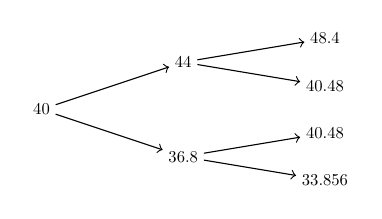
\begin{tikzpicture}[->, level/.style={sibling distance = 2cm/(#1), level distance = 3cm}, scale=0.6,transform shape,grow=right]
      \node {40}
        child {node {36.8}
          child { node {33.856} }
          child { node {40.48} }
        }
        child {node {44}
          child { node {40.48} }
          child { node {48.4} }
        };
    \end{tikzpicture}
  \end{center}
  For this European put option we have that the pay-out is $Y_T(\omega)=g(S_T(\omega))=\{42-S_T(\omega)\}_+$ for each $\omega\in\Omega$ and $0$ for all other $t$. I summarise the pay-outs in the tree below
  \begin{center}
    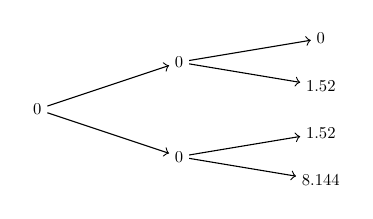
\begin{tikzpicture}[->, level/.style={sibling distance = 2cm/(#1), level distance = 3cm}, scale=0.6,transform shape,grow=right]
      \node {0}
        child {node {0}
          child { node {8.144} }
          child { node {1.52} }
        }
        child {node {0}
          child { node {1.52} }
          child { node {0} }
        };
    \end{tikzpicture}
  \end{center}
  The time $t=0$ value for this European put option is
  \[\begin{array}{rcl}
    \Pi(0)&=&\frac1{(1+r)^T}\sum_{n=0}^T{T\choose n}q^n(1-q)^{T-n}g(S_0u^nd^{T-n})\\
    &=&\frac1{1.03^2}\sum_{n=0}^2{2\choose n}\frac{11^n7^{2-n}}{18^2}\left\{42-S_0u^nd^{T-n}\right\}_+\\
    &=&\frac1{1.03^2}\sum_{n=0}^1{2\choose n}\frac{11^n7^{2-n}}{18^2}\left\{42-30\cdot(1.1)^n\cdot(0.92^{2-n})\right\}_+\\
    &=&\frac1{1.03^2}\left(1\cdot\frac{7^2}{18^2}\cdot8.144+2\cdot\frac{11\cdot7}{18^2}\cdot1.52\right)\\
    &\simeq&1.84194\dots
  \end{array}\]
\end{answer}

\begin{question}{3. b)}
  A six-month American put option with a strike price of £42?
\end{question}

\begin{answer}{3. b)}
  The price process $S_t$ is the same as described in \texttt{3. a)}. For this American put option we have that the pay-out is $Y_t(\omega)=\{42-S_t(\omega)\}_+$ for each $t=0,1,2,3$ and $\omega\in\Omega$. I summarise the pay-outs in the tree below
  \begin{center}
    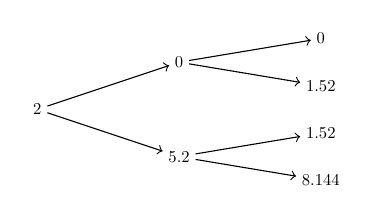
\begin{tikzpicture}[->, level/.style={sibling distance = 2cm/(#1), level distance = 3cm}, scale=0.6,transform shape,grow=right]
      \node {2}
        child {node {5.2}
          child { node {8.144} }
          child { node {1.52} }
        }
        child {node {0}
          child { node {1.52} }
          child { node {0} }
        };
    \end{tikzpicture}
  \end{center}
  I will now construct a Snell Envelope $\{Z_t\}$ for the payoff process $\{Y_t\}$.
  \par By definition, $Z_2(\omega)=Y_2(\omega)\ \forall\ \omega\in\Omega$.
  \par Let $\omega_u,\omega_d$ represents the events the price of underlying asset increases/decreases during the first time-step, respectively.
  \par Consider time-period $t=1$ and that the event $\omega_u$ has occurred. Then
  \[ \expect[Z_2|\mathcal{F}_1]=q\cdot0+(1-q)\cdot1.52=\frac{11}{18}\cdot0+\frac7{18}\cdot1.52=0.5911 \]
  Thus, given $\omega_u$ occurred, we can deduce $Z_1$
  \[\begin{array}{rrl}
    Z_1&:=&\max\{Y_1,\expect[Z_2|\mathcal{F}_1]\}\\
    &=&\max\{0,0.5911\}\\
    &=&0.5911
  \end{array}\]
  \par Consider time-period $t=1$ and that the event $\omega_d$ has occurred. Then
  \[ \expect[Z_2|\mathcal{F}_1]=\frac{11}{18}\cdot1.52+\frac7{18}\cdot8.144=4.096 \]
  Thus, given $\omega_d$ occurred, we can deduce $Z_1$
  \[\begin{array}{rrl}
    Z_1&:=&\max\{Y_1,\expect[Z_2|\mathcal{F}_1]\}\\
    &=&\max\{5.2,4.096\}\\
    &=&5.2
  \end{array}\]
  \par Consider time-period $t=0$. The
  \[ \expect[Z_1|\mathcal{F}_0]=\expect[Z_1]=\frac{11}{18}\cdot0.5911+\frac7{18}\cdot5.2=2.3834 \]
  We can deduce $Z_0$
  \[\begin{array}{rrl}
    Z_0&:=&\max\{Y_0,\expect[Z_1|\mathcal{F}_0]\}\\
    &=&\max\{2,2.3834\}\\
    &=&2.3834
  \end{array}\]
  The time $t=0$ fair price of this American Option is 2.3834.
\end{answer}

\begin{question}{4.}
  What is the price of a European call option on a non-dividend paying stock when the stock price is £69, the strike price is £70, the risk-free interest rate is 6\% per annum, the volatility is 35\% per annum, and the time to maturity is six months?
  \par What is the price of a European put option with the same strike price?
\end{question}

\begin{answer}{4.}
  \everymath={\displaystyle}
  In this problem we have that
  \[ S_0=69\quad K=70\quad r=0.06\quad \sigma^2=0.35\quad U=1/2 \]
  $U$ is defined to equal 1/2 as the interest rate is defined over a year but the option matures in six months.
  \par By the Black-Scholes formula we have that the time $t=0$ fair price for this European call option is
  \[\begin{array}{rrrl}
    &\Pi^{BS}(0)&:=&S_0\Phi\left(d_1(S_0,U)\right)-Ke^{-rU}\Phi\left(d_2(S_0,U)\right)\\
    &&=&69\Phi\left(d_1(69,1/2)\right)-70e^{-0.03}\Phi\left(d_2(69,1/2)\right)\\
    \text{where}&\\
    &d_1(s,u)&:=&\frac{\ln(s/K)+(r+\sigma^2/2)U}{\sqrt{\sigma^2U}}\\
    \implies&d_1(69,1/2)&=&\frac{\ln(69/70)+(0.06+0.35/2)\cdot(1/2)}{\sqrt{0.35\cdot(1/2)}}\\
    &&=&0.2468\dots\\
    \text{and}\\
    &d_2(s,u)&:=&\frac{\ln(s/K)+(r-\sigma^2/2)U}{\sqrt{\sigma^2U}}\\
    \implies&d_2(69,1/2)&=&\frac{\ln(69/70)-(0.06+0.35/2)\cdot(1/2)}{\sqrt{0.35\cdot(1/2)}}\\
    &&=&-0.1718\dots
  \end{array}\]
  Note that
  \[ \Phi(0.2468)=0.597\quad\text{and}\quad\Phi(-0.1718)=0.432 \]
  Thus
  \[ \Pi^{BS}(0)=69\cdot0.597-70\cdot0.432=10.432 \]
  The time $t=0$ fair-price for this European call option is 10.432.
  \par I will now determine the time $t=0$ price for the equivalent European put option.
  \par The Put-Call parity states that
  \[ S_0+P_0-C_0=Ke^{-rT} \]
  Thus, in this problem we have
  \[\begin{array}{rrcl}
    &69+P_0-10.432&=&70e^{-0.06/2}\\
    \implies&P_0&=&9.363
  \end{array}\]
  The time $t=0$ fair-price for the equivalent put option is 9.363.
\end{answer}

\end{document}
